\section{Literature review}\label{sec:literature}
% 
% Introduction to literature review
% 
We can overally conclude that concept of platooning is a heavily researched area. The articles regarding vehicles driving in strings, range as back as the eighties \cite{Peppard1974StringSystems}.
Since then the research has been divided into two major areas, as described by \cite{Vinel2015Vehicle-to-vehicleScenarios}. First area is the \emph{Cooperative adaptive cruise control} and the second one is \emph{platooning}. While both touch the scope of our project and should be researched, we focused mainly on the latter one.\par
% 
In this chapter we review some of the most recent and most significant works. Two of them are \acrshort{sartre} \cite{Chan2012ProjectSARTRE} and Safespot \cite{Safespot}, both supported by the European Commission. Then chapter continues by discussing the inter-vehicular connectivity and Companion \cite{2016CompanionProject} project afterwards.\par
% 
At the end of the chapter, examples of other works are shown, to describe some of the challenges researched in connection with Platooning.

\subsection{\textit{SARTRE}}\label{sec:SARTRE}

% /include SARTRE notes from Michal/
% \par
SARTRE \cite{Chan2012ProjectSARTRE} stands for Safe Road Trains for the Environment and it is a project which is financed by the European Union. The project is already finished, it lasted for 36 months since September 2009. Its goal was to develop a prototype of system that would be able to coordinate road-trains, so called platoons, in a way that only the first car in a platoon must be driven by a driver and all others are just following it without a need of a driver to pay attention on road. Very important for this project was the use of available technologies meaning that the system may be (in theory) implemented straight after finishing the study. Also, it was designed to work on the actual roads without the need of changing the infrastructure.\par
% 
There have been reasons for realisation of such a project. The traffic on roads is heavier every year, meaning that there are more and more cars being driven which raises several problems: pollution, safety, traffic congestion and limited space for increasing the road capacity. These were the main reasons for realisation of SARTRE. \par
% 
As already mentioned, the main goal was to develop system that would be able to handle platooning. The idea is that in the first vehicle (so called lead vehicle - LV) would be a trained driver which is followed by other vehicles (following vehicles - FV) that after joining a platoon become fully autonomous. Therefore, there are three categories of vehicles with which the system would interact: lead, following and other non-platooning vehicles. The reason is that platoons would be driving down the normal highways mixed with normal (non-platooning) traffic. The system must be able to handle this as there may many cases of direct interaction of the platoon with other vehicles (a vehicle interrupting the platoon by breaking in between two cars, etc.). This however, has not been covered deeply by this project, they are just aware that different situations of interaction may occur and that they must be handled.\par
% 
The architecture of the system was not described to details, there has just been diagrams showing how it looked like (Figure \ref{fig:HW_FW}, showing the hardware configuration of the following vehicle, and Figure \ref{fig:HW_LW}, the configuration of leading vehicle). Also, it was not mentioned what kind (brand, model) of hardware has been used.\par
% 
\begin{figure}[t]
    \centering
    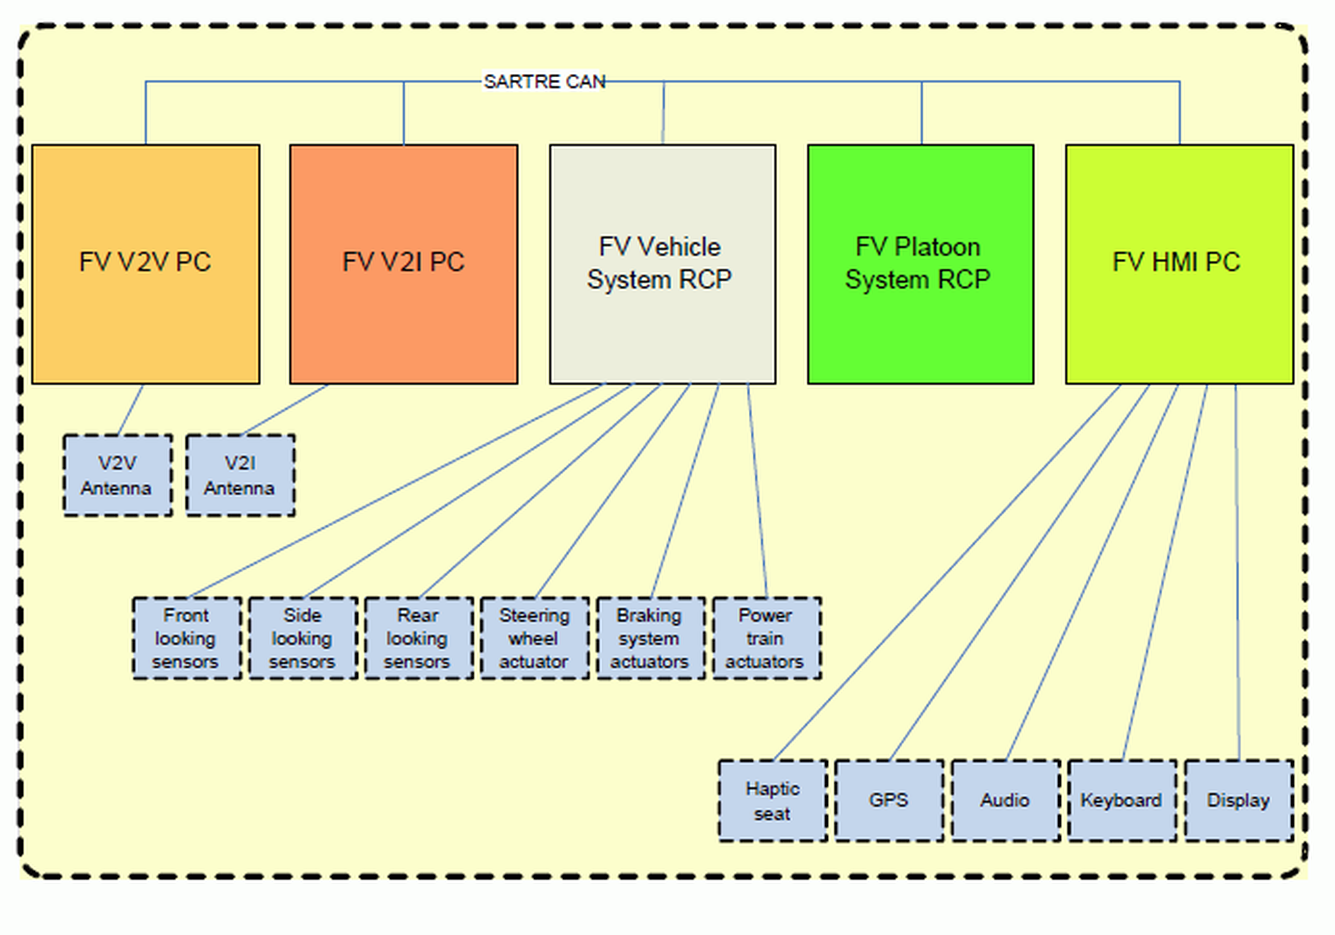
\includegraphics[width=.95\textwidth]{HW_FW}
    \caption{Hardware architecture of following vehicle (vehicle that is platooning). Taken from \cite{Chan2012ProjectSARTRE}.}
    \label{fig:HW_FW}
\end{figure}
% 
\begin{figure}[t]
    \centering
    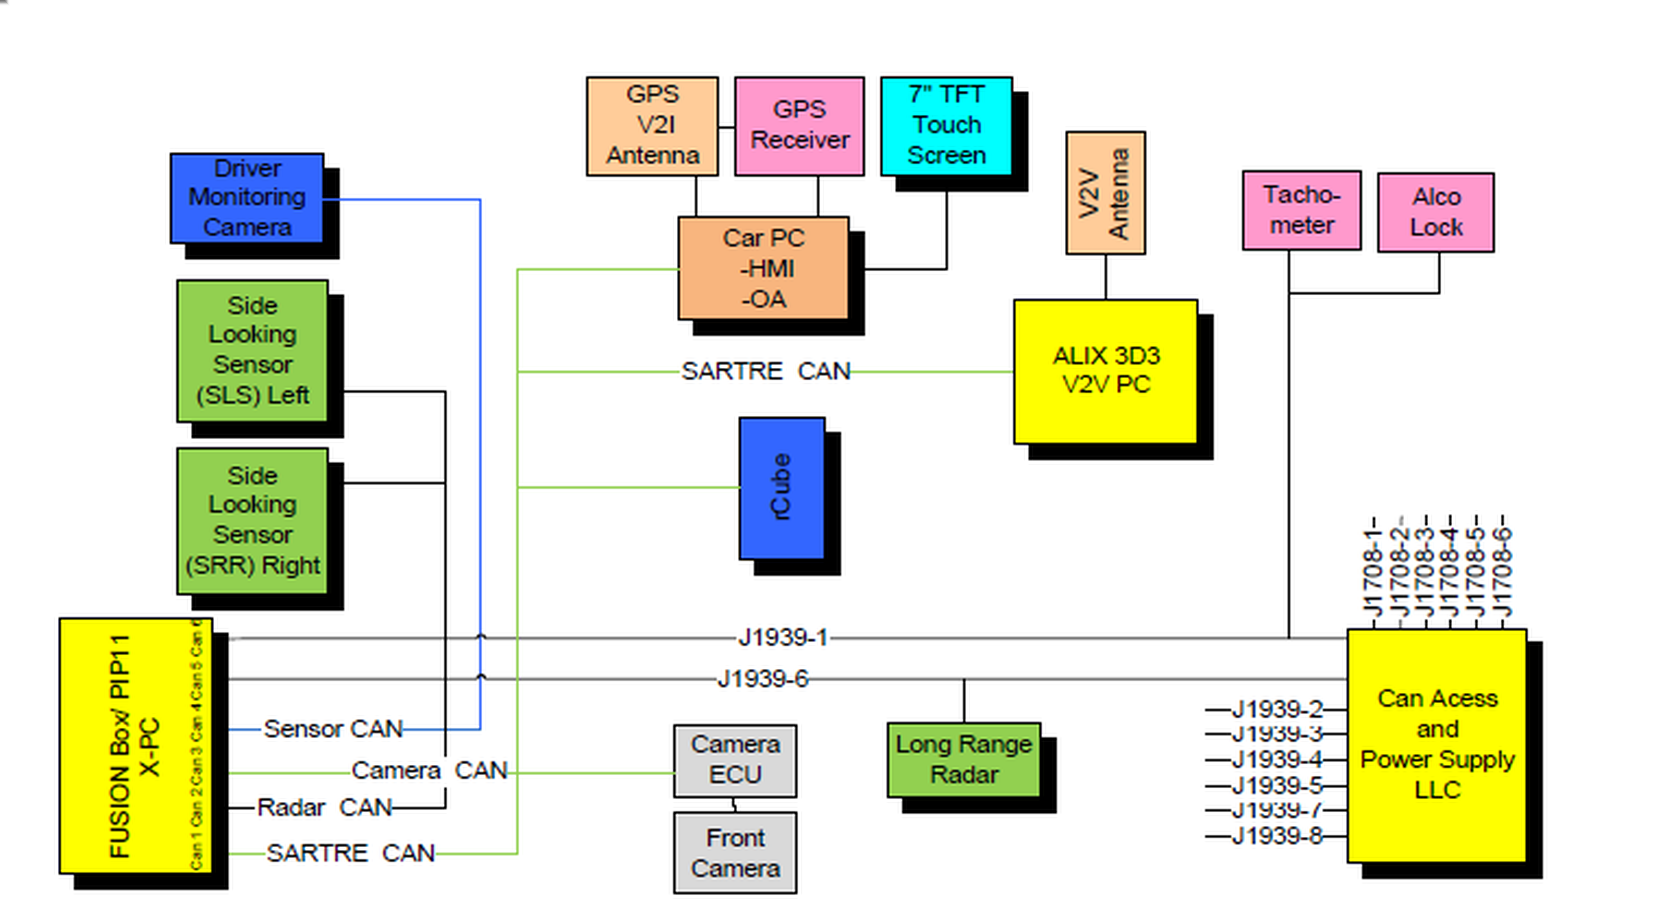
\includegraphics[width=.95\textwidth]{layoutHW}
    \caption{Hardware architecture of the leading vehicle. Taken from \cite{Chan2012ProjectSARTRE}.}
    \label{fig:HW_LW}
\end{figure}
% 
At the end the testing was conducted with truck as the leading vehicle and another truck and three cars as following vehicle. It successfully shown that it is possible to create a platoon of several vehicles where the following vehicles were driven autonomously. Also, that the fuel consumption is being reduced by approximately 10\%.

\subsection{\textit{SAFESPOT}}
In 2006 a project running for 4 years called SAFESPOT \cite{Safespot} was co-funded by the European Commission Information Society and Media, and had an objective to improve road safety. One of the key elements was to have vehicles exchange data between them and with infrastructure (V2V and V2I) to advice or warn the driver of upcoming situation happening.\par
% 
\subsubsection{Architecture}
SAFESPOT is composed of nodes, that communicates with each other through short range wireless communication called VANET (Vehicle Ad-hoc NETwork) using \hyperref[sec:802.11p]{IEEE 802.11p} as physical layer. A node can be in a vehicle or on an infrastructure such as a traffic light. All nodes create data through their sensors or through data from other nodes and are then collected in a multi-layered Database named Local Dynamic Map (LDM).
LDM consist of 4 layers. From bottom up, the first is the static map like Google maps. The second is Landmarks, such as road signs, trees, buildings etc. The third is temporary objects that can change from day to day, such as road work. And lastly Dynamic object which is immediate status, such as congestion, current traffic light colour etc. \cite{Brignolo2008UseProject}.
To locate the position of the vehicles, SAFESPOT uses the road data from GPS, road landmark recognition and dead reckoning\footnotemark.\par
%
% 
\footnotetext{\textquote[Taken from: \url{https://en.wikipedia.org/wiki/Dead_reckoning}]{\textit{In navigation, dead reckoning or dead-reckoning is the process of calculating one's current position by using a previously determined position, or fix, and advancing that position based upon known or estimated speeds over elapsed time and course.}}}
% 
% 
The data rate and communication channel usage is restricted and is one of the physical bottle neck in the system. US WAVE standard (which is similar to SAFESPOT) has a specified data rate of:
\begin{itemize}[noitemsep]
    \item Remote On Board Unit (vehicle): 2320 bit/s
    \item Remote Road Side Unit (traffic light): 22500 bit/s  
\end{itemize}
Though the numbers might be slightly different in Europe, it still shows the bottleneck that exists in this kind of communication channel, especially for On Board Units.\par
% 
Depending on how advanced we want the platooning to be, will lessen the amount of data and how accurate it needs to be. Since SAFESPOT main objective was safety, they needed as many details as possible, to make sure that the driver was given the correct information to avoid a incoming crash. If we want to make platooning only available on highways and only the speed and the brake being controlled, the amount of information needed to be sent to the “VANET” is severely lessened, but if everything were to be automatized, at least as much data as SAFESPOT is needed. The restriction of the data rate is something to take into consideration as well. 

\subsection{\textit{Vehicular Networks}}

% 
Vehicular Ad Hoc Networks (VANETs) are gaining significant amount of interest in educational studies and industry. It is believed that implementation of V2V and V2I communications will lead to success in transportation business in a near future. A report established by Caixing Shao and Supeng Leng from University of Electronic Science and Technology in China \cite{Shao2014AnalysisNetworks} analyses VANET probability in a platoon in a detailed manner.\par
% 
Their V2I solution is tightly coupled with RSU (Road Side Units) implementation on the roads. A problem we are solving in this project is mostly dependant on successful V2V communication and is not meant to be dependant on road infrastructures. With that in mind continuous V2I communication is not necessary for this project, but having some V2I (e.g. in order to facilitate periodical Internet connection) would definitely be beneficial for planning and user experience.\par
% 
Analysis made in University of Electronic Science and Technology in China offers an intelligent solution for continuous Internet access through road side units even if the vehicle is not in the range of RSU. It would use platoon vehicles as relays to reach access to Internet. It is an idea that has potential to be implemented worldwide, so we decided to dig further.\par
% 
Since our platoon solution is not dependant on continuous V2I communication and RSUs are not being implemented in a big scale at the moment \cite{Tonguz2013CarsSolution}, we researched the core idea of using other vehicles in the platoon as relays. Keeping in mind that cars in the platoon will have V2V connection anyways. We have found an interesting report made by students of Carnegie Mellon University in Thailand \emph{Cars as Roadside Units} \cite{Tonguz2013CarsSolution}.\par
% 
Their idea is based on vehicles adopting new wireless communication technology, that is intentionally developed for V2X (Vehicle to everything) - DSRC (Dedicated Short Range Communication) \cite{OfficeoftheAssistantSecretaryforResearchandTechnologyIntelligentSheet}.
Report is proving that implementing RSUs widely might be too costly and inefficient, so they suggest using DSRC enabled vehicles as temporary Road Side Units on a planned briefly stops during the trip. Since the car is acting as RSU for short period of time it would mostly be used to send out messages in case of accident or congestion in ROI (range of interest).

\subsection{\textit{Companion}}\label{sec:Companion}
% 
A very influential research project for platoon implementation in near future, named \emph{Companion} \cite{2016CompanionProject} has been established by SCANIA between 2013 and 2016. Project was coordinated by Magnus Adolfson and involved such automotive giant as Volkswagen.\par
% 
Project's full definition is: \textquote[\footnotemark]{\textit{Cooperative dynamic formation of platoons for safe and energy-optimised goods transportation}} and it is concentrated on research and development of mobility technologies for supervised platooning. Companion's main objective is to improve fuel efficiency and safety of transportation.%
% 
\footnotetext{\url{http://cordis.europa.eu/project/rcn/110628_en.html}, accessed 10/04/2017}%
% 
Problems that are analysed by Companion, are closely related to the ones we are trying to solve with our road train solution in this project and it seems worthwhile investigating work done by experts in the field\footnotemark.\par
% 
\footnotetext{\url{https://youtu.be/_19ui-8f8cw}, accessed 10/04/2017}
% 
Solution suggested by Companion is somewhat new comparing to other platoon projects. They want to form platoons dynamically - meaning vehicle could join and leave platoon whenever it is suitable for that particular vehicle. Participant doesn't have to stay in the platoon for the whole trip, every vehicle can plan different starting and destination locations. Cars would use V2V communication to be able to find nearest platoons and then when in platoon mode, vehicles would communicate constantly to steer, brake and accelerate following vehicles (FV). It is a solution that is not dependant on road infrastructure. Also worth mentioning that project was mostly focused on heavy-duty vehicles.\par
% 
Scope for the project Companion was development and prototype implementation of \emph{Off-Board system for Platoon Coordination} and \emph{On-Board System for Coordinated Vehicle Platooning}.\par
% 
\emph{Off-Board system} will consist of route calculation and optimisation engines and off-board HMI. The system would be controlled by remote dispatchers and is most suitable for planning long distance goods transportation.\par
% 
For developing \emph{On-Board V2V system} interviews with drivers took place. They covered drivers' opinions on vehicle HMIs and platooning in general. Results showed that drivers are positive about new technologies and idea of platooning. Although they would have to build trust of the system for short-distance driving.\par
% 
It is fair to conclude that Companion project was successful in sense that it proved platoon to be high potential and near future technology. Physical and practical tests showed that it could lower fuel consumption up to 12.6\%. Various simulations and driver interviews showed that platooning could drastically improve safety and congestion problems on the roads. Results of various simulations and tests established during Companion project will be analysed more in depth in \hyperref[sec:data]{\textit{Empirical data} section} in this project.
% 

\subsection{\textit{A review of Truck Platooning Projects for Energy Savings}}

This paper \cite{Tsugawa2016ASavings}, published in \emph{Transacions on Intelligent Vehicles}, an IEEE journal, serves as a review of platooning projects that has been done over past decades. Also, it serves as an overview of what platooning is, why there has been projects done since 1950s, what are the objectives of automated platooning and what technologies/projects has been developed since (the most notable once according to authors).
This paper classifies objectives of platooning to three main categories: Energy consumption an CO2 emission, characteristics of the trucking industry and transportation capacity. However, they also realise other positive aspects of it such as safety increase, congestion reduction and comfort.\par
% 
Projects being described in the paper are Automated Trucks in Energy ITS, Electronically Coupled Truck Platoons “KONVOI”, PATH Development of Truck Platooning and CACC Systems. The purpose of each project is being described there along with how it works. Longitudinal controls and system of each project was described there in details as well as its lateral controls and system. The architecture of each system was presented, showing all components of the system and their interaction with each other. For communication between trucks, V2V communication is being used and all of its components are being presented, as well as what information are send/received and what is payload (in some projects, are these information available).\par
% 
The last section of this paper is about impacts of platooning. There are presented findings of the previously mentioned project. Those findings are mostly showing about fuel savings at different gaps between truck.\par
% 
This paper helped us to get better understanding of platooning as it compares several project’s main ideas, aims, technology and findings. Because of that, we were able to get a lot of secondary data for our project, without a need for going through each project separately as all necessary data are presented there.



% Book: Fuel-efficient heavy-duty vehicle platooning
\subsection{\textit{Fuel-efficient heavy-duty vehicle platooning}}
The thesis by Alam A. \cite{Alam2014Fuel-efficientPlatooning}, which was later published also as a book poses as a very valuable resource for this project. The author recognises the growing need of solving the road congestion problem and the persistent need of fuel savings. In the thesis author investigates how the platoons, formed of HDVs (Heavy duty vehicles), can be designed, implemented and what the parameters for optimal fuel savings, while maintaining reasonable level of safety, are.\par
% 
% 
The experiments have been performed with a platoon of three similar HDVs, with 90km long test runs on a highway in Sweden. Fuel consumption was being measured, first, while vehicles were driving alone, and later, while driving in platoon. The test runs were conducted multiple times over period of 5 days to rule out the influences of weather and other variables. The findings show that fuel reduction between 3.9\% and 6.5\% can be obtained for vehicles in the platoon, depending on the weight of the vehicles. Another major influence on the fuel savings is the road gradient. The test runs showed, that with greater road gradient the efficiency of the platoon drops. Reasons for this is the limited engine power and other system dynamics that have not been accounted for, such as gear changes. The thesis also concludes, that it is possible to operate a platoon with inter-vehicular distances between 1-2 meters while maintaining safe operation. Smaller distances could be possibly achieved with more powerful breaks and shorter delays in communication. Furthermore, due to the lack of detailed research, it is concluded that \textquote[\cite{Alam2014Fuel-efficientPlatooning}]{It is still unclear how the unmodeled nonlinearities, such as gear changes, brake dynamics, engine dynamics, and a varying road topography affect the control performance in practice.}
\par
% 
Two models are investigated for controlling the behaviour of the platoon. First, \emph{decentralised} model investigates how the platoon could work, if there is no central control node, but rather each vehicle only communicates with the vehicles surrounding it. The second, \emph{look-ahead control} model describes, how to account for differences among vehicle mass and engine power, which become critical for efficient operation of a platoon in steep road sections, by adjusting the speed of a vehicle prior to approaching a steep road segment.
\par
% 
Technology-wise, the thesis is not very detailed. It states, the the test vehicles are equipped with wireless control unit, which uses IEEE 802.11p standard for communication. Furthermore, GPS and a \enquote{standard doppler radar}. We will further investigate the use of these technologies.
% 
% 
%
% IEEE journal article: Cooperative look-ahead control for fuel-efficient and safe heavy-duty vehicle platooning
\subsection{\textit{Cooperative look-ahead control for fuel-efficient and safe heavy-duty vehicle platooning}}
% 
This article \cite{Turri2016CooperativePlatooning} published in IEEE journal, similarly as \cite{Alam2014Fuel-efficientPlatooning}, considering only HDVs as members of the platoon, investigates how slopes influence the effectiveness of the platoon. It further investigates models that could be used to increase the fuel efficiency of the platoons in hilly areas.
\par
% 
It compares the three approaches to driving vehicles in a group: \emph{Cruise Control} (CC), \emph{Look-ahead cruise control} (LACC) and \emph{Cooperative look-ahead cruise control} (CLAC), each with different rules regarding the control of vehicles' speed. The CLAC is considered as most effective method, as it provides all members of the platoon with sufficient information about road ahead, so they can adjust their own speed accordingly. The CLAC introduces new layer into the platooning, denoted as \emph{platoon coordinator} layer. Such layer \textquote[\cite{Turri2016CooperativePlatooning}]{is responsible  for  the  coordination  of  the  platoon  by  defining a speed profile that is feasible and fuel-efficient for the entire platoon  by  exploiting  preview  topography  information}.
\par
% 
% 
% 
% Vehicle Platoon Formation Using Interpolating Control (article) from AAU
\subsection{Other works}
% 
Number of works, like \cite{Alvarez1997SafeSystems}, \cite{Nowakowski2015CooperativeAlternatives} focus on the system from higher perspectives and discuss, what the overall goal of the system is, what in involves, how it should be used to ensure safety of the traffic and what the architecture of such system should be. Some of the works \cite{Larsson2015TheHeuristics}
approach the problem of platooning from the perspective of mathematics and algorithmization. They try to answer the questions of ideal vehicle routing on (inter-)national scale, in order to optimise the flow of the vehicles and create best strategies for formation of the platoons.
Another important aspect for the problem is how to maximise the fuel savings. Journal article \cite{Turri2016CooperativePlatooning} investigates the changes in the fuel savings in hilly terrain and how to optimise the algorithms of platooning vehicles (trucks) in areas, where they have to break and accelerate often.\par
% 
\subsubsection{\textit{Vehicle Platoon formation}}
The article \cite{Tuchner2015VehicleControl} shows how it is possible to solve the problem of platooning through regulating the vehicles speed and spacing between them with the use of math and algorithms. 3 different solution is being compared with Interpolation Control, Improved Interpolation Control and Model Predictive Control. The differences in result can be found in the article.\par
%No idea how the math works, but at least we can reference to this, when talking about that its not only data between the vehicles, but also alot of math running in the background. 
% 

\subsection{Conclusion}
% Write summary of literature review
The key findings in this chapter, besides the fact that there is a lot of research material about the subject, are:
\begin{itemize}[noitemsep]
    \item There are systems developed, where \acrlong{CACC} (crucial part of platooning) has been successfully tried out and tested. Most of the vehicles used \acrshort{GPS}, some kind of wireless communication and a radar to determine distance from vehicles in front.
    \item There are fuel savings, while platooning, for all vehicles - both leading and following vehicles. These savings depend on distance of the vehicles and slope of the road.
    \item Different models can be used for controlling the operation of the platoon, from the perspective of fuel savings and usability (how vehicles join platoons, how two platoons can merge).
\end{itemize}
% 
We have reviewed some of the most significant works concerning platooning, including comprehensive EU-founded projects like \acrshort{sartre} or Companion. As the research progressed, we kept finding more and more material of great informational value, ranging from detailed technical challenges of the standards used in vehicular environments to broader aspects of platooning. Naturally, not all of them can be listed in this chapter and/or reviewed in great detail. Material listed here, however, gives a good picture of the state of the art within the field up to date. Our focus for the next part of this report will be put on determining the stakeholders and their requirements for the platooning concept.\par
